\documentclass[]{article}
\usepackage[utf8]{inputenc}
\usepackage[english,russian]{babel}
%\usepackage[12pt]{extsizes}
\usepackage{amsmath}
\usepackage{enumerate}

%\usepackage[left=3cm, top=1.5cm, right=1.3cm, bottom=2cm, nohead, footskip=10mm]{geometry}
\usepackage[12pt]{extsizes}
\linespread{1.3}
\usepackage[left=3cm, top=1.5cm, right=1.3cm, bottom=2cm, nohead, footskip=10mm]{geometry}


\usepackage[absolute,overlay]{textpos}
\usepackage{indentfirst}
\usepackage{float}
\restylefloat{table}
\usepackage{hyperref}
\usepackage{mathtext}
\usepackage{amsfonts}
\usepackage{amsthm}
\usepackage{tikz}
\usepackage{xspace}
\usetikzlibrary{shapes,positioning,shadows,trees,automata,arrows.meta,shapes.geometric}
\usepackage{pgf-pie}
\usepackage{chngcntr}
\usepackage{pdfpages}
\usepackage{systeme}
\usepackage{empheq}
\numberwithin{equation}{section}
\usepackage{caption}
\DeclareCaptionLabelSeparator{none}{. }
\captionsetup{labelsep=none}


\pagestyle{plain}

\begin{document}
    \thispagestyle{empty}
	\begin{center}
        Министерство образования и науки Российской Федерации\\
		Санкт-Петербургский государственный технический университет\\
		Институт прикладной математики и механики\\
		Кафедра <<Телематика>>\\
		\vspace{5cm}
		\textbf{\textbf{ЛАБОРАТОРНАЯ РАБОТА}}\\
        \vspace{0.5cm}
        \textbf{ПО ТЕМЕ}\\
        \vspace{0.5cm}
		\textbf{\textbf{<<Деревья решений>>}}\\
		\vspace{3cm}
		по направлению 02.04.01.02 <<Организация и управление суперкомпьютерными системами>>
	\end{center}
	\vspace{2cm}
	\begin{tabular} {l l l}
	\hspace{9.5cm} & Выполнил: & \\
	& Студент гр. 13643.1 & Титов А.И.\\
	& Проверил: & Уткин Л.В.
	\end{tabular}
	\vspace{4.5cm}
	\begin{center}
		Санкт-Петербург\\
		2019
    \end{center}


	\renewcommand\contentsname{Оглавление}
	\tableofcontents

    \newpage
    \section*{Постановка задачи}
    \addcontentsline{toc}{section}{Постановка задачи}
    \vspace{-0.1cm}
    Требуется выполнить следующие задачи:
    \begin{enumerate}
        \item Загрузить набор данных Glass из пакета “mlbench”. Построить дерево классификации для модели, задаваемой следующей формулой: $Type \sim.$  , дайте интерпретацию полученным результатам. При рисовании дерева использовать параметр cex=0.7 для уменьшения размера текста на рисунке. Выявить, является ли построенное дерево избыточным. Выполнить все операции оптимизации дерева.
        Определить, к какому типу стекла относится экземпляр с характеристиками:

        RI =1.516 Na =11.7 Mg =1.01 Al =1.19 Si =72.59 K=0.43 Ca =11.44 Ba =0.02 Fe =0.1
        \item Загрузить набор данных spam7 из пакета DAAG. Построить дерево классификации для модели, задаваемой следующей формулой: $yesno \sim.$, дать интерпретацию полученным результатам. Запустить процедуру “cost-complexity prunning” с выбором параметра k по умолчанию, method = ’misclass’, вывести полученную последовательность деревьев. Выявить, какое из полученных деревьев является оптимальным.
        \item Загрузить набор данных nsw74psid1 из пакета DAAG. Построить регрессионное дерево для модели, задаваемой следующей формулой: $re78 \sim.$.
        \item Загрузить набор данных Lenses Data Set из файла Lenses.txt:
            \begin{itemize}
                \item 3 класса (последний столбец):\\
                1 : пациенту следует носить жесткие контактные линзы;\\
                2 : пациенту следует носить мягкие контактные линзы;\\
                3 : пациенту не следует носить контактные линзы.
                \item Признаки (категориальные):\\
                \textbf{Возраст пациента}: (1) молодой, (2) предстарческая дальнозоркость, (3) старческая дальнозоркость;\\
                \textbf{Состояние зрения}: (1) близорукий, (2) дальнозоркий\\
                \textbf{Астигматизм}: (1) нет, (2) да\\
                \textbf{Состояние слезы}: (1) сокращенная, (2) нормальная
            \end{itemize}
            Построить дерево решений. Какие линзы надо носить при предстарческой дальнозоркости (2), близорукости (1), при наличии астигматизма (2) и сокращенной слезы (1)?
        \item Для построения классификатора используйте заранее сгенерированные обучающие и тестовые выборки, хранящиеся в файлах svmdata4.txt, svmdata4test.txt.
        \item Разработать классификатор на основе дерева решений для данных Титаник (Titanic dataset).
    \end{enumerate}

    \newpage
    \section{Набор данных <<Glass>>}
        Для обучающего множества было построено дерево решений (рис. 1). При отсутствии ограничений на глубину дерева и 20 терминальных вершинах в качестве максимального количества терминальных вершин было выявлено, что приведенный пример принадлежит второму классу с вероятностью $\approx 0.83$.

        \begin{figure}[H]
            \centering
            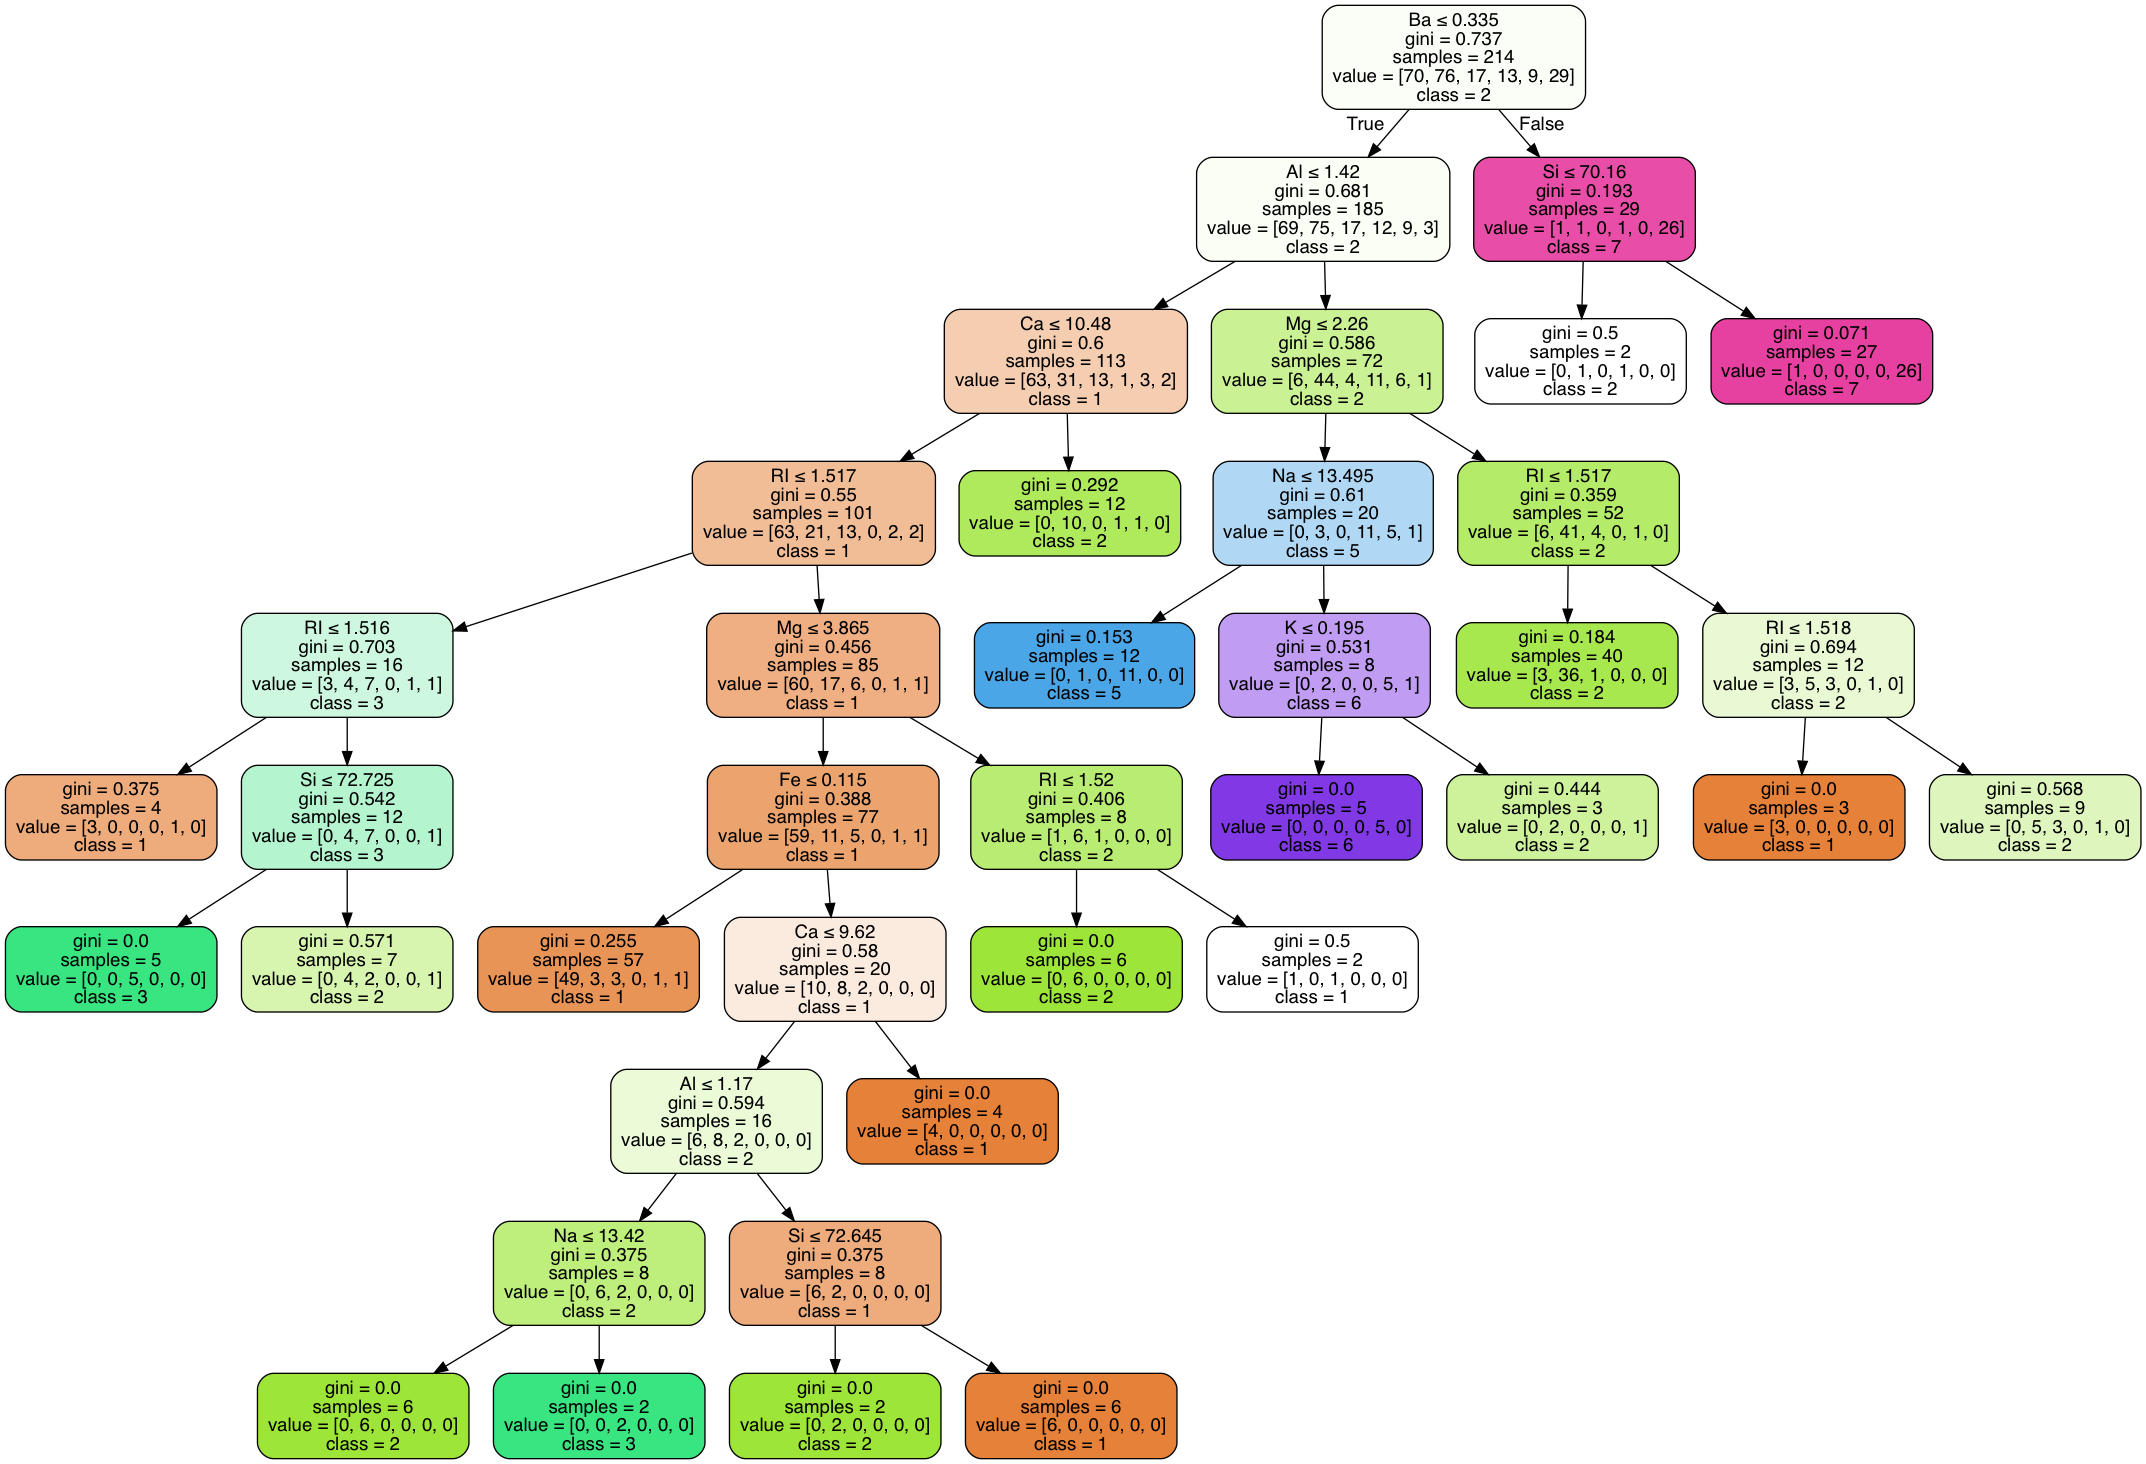
\includegraphics[width = 1.0\linewidth]{data/glass_tree_full.png}
            \caption{Дерево решений для примера <<Glass>>}
        \end{figure}

        Однако ограничив глубину дерева до 4ех было достигнуто значение вероятности 1.0. При этом появилась возможность сократить количество терминальных вершин до 17ти (рис. 2).

        \begin{figure}[H]
            \centering
            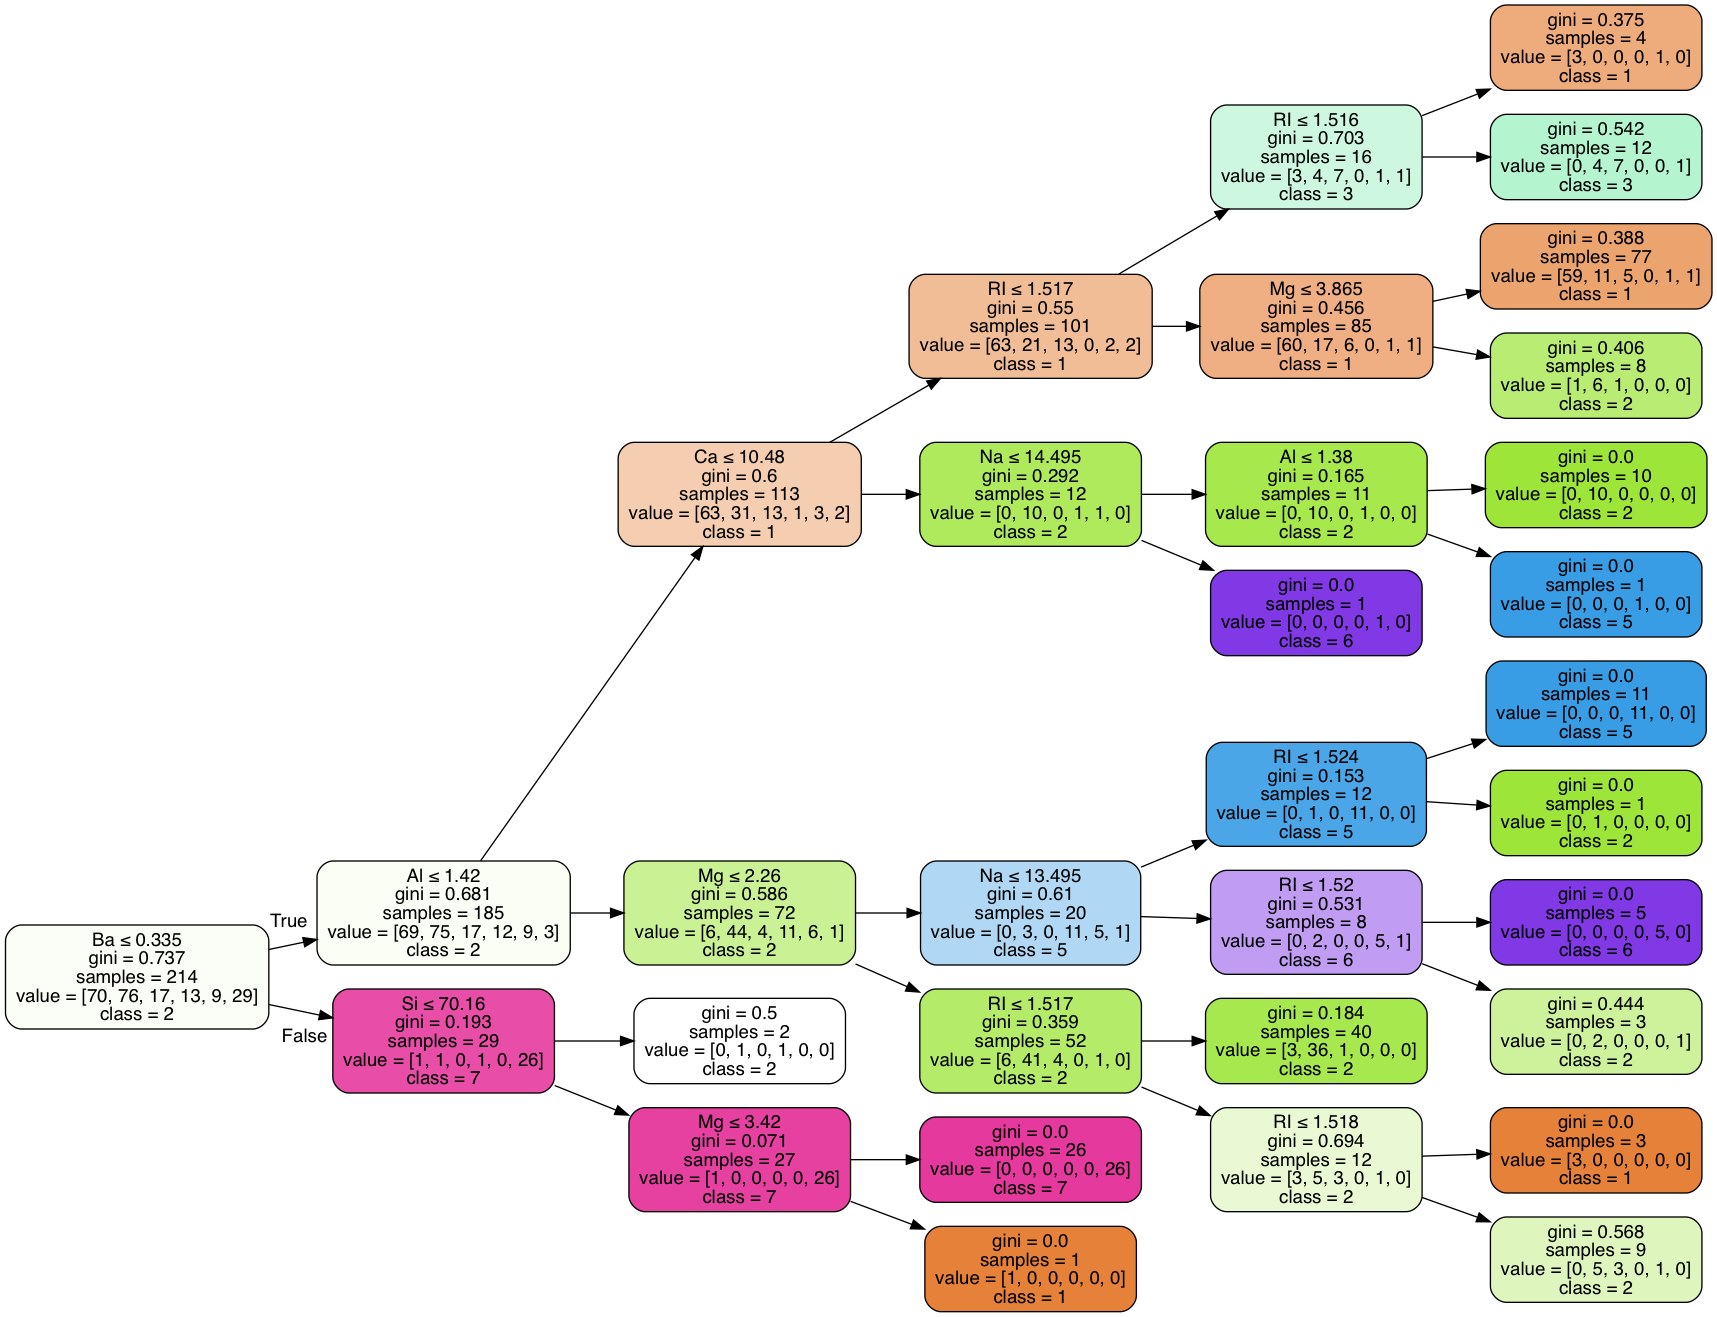
\includegraphics[width = 1.0\linewidth]{data/glass_tree_opt.png}
            \caption{Усеченное дерево решений для примера <<Glass>>}
        \end{figure}

    \section{Набор данных <<spam7>>}

        Было построено дерево решений (рис. 3).

        \begin{figure}[H]
            \centering
            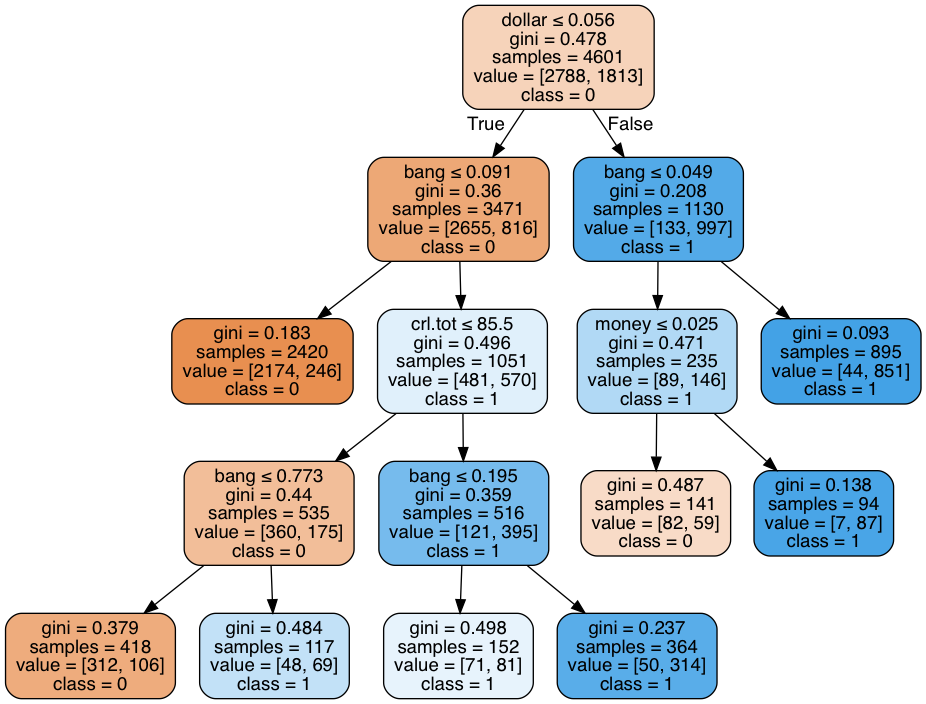
\includegraphics[width = 0.75\linewidth]{data/spam7.png}
            \caption{Дерево решений для примера <<spam7>>}
        \end{figure}
        \vspace{-0.5cm}
        Для того, чтобы определить наиболее удачное количество терминальных вершин был построен график зависимости ошибочных предсказаний от количества терминальных вершин (рис. 4). Проанализировав график можно сделать вывод, что наилучшим выбором будут значения от 5 до 7. Далее анализируя результаты экспериментов было выбрано значение 6 в качестве оптимального.
        \vspace{-0.5cm}
        \begin{figure}[H]
            \centering
            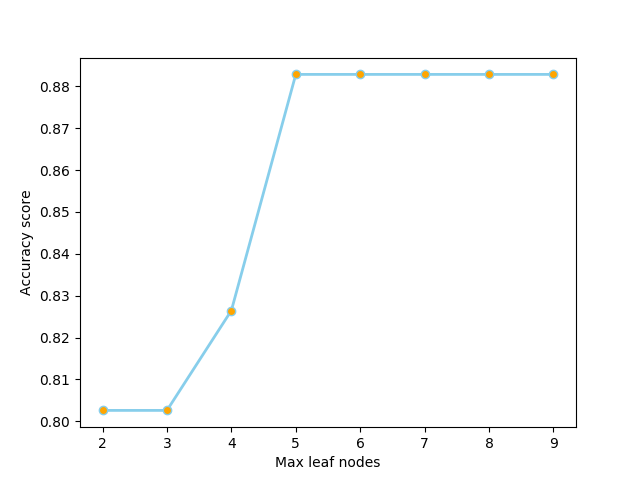
\includegraphics[width = 0.7\linewidth]{data/spam7_stat.png}
            \caption{График зависимости числа ошибок от количества терминальных вершин}
        \end{figure}

        Полученное дерево изображено на рисунке (рис. 5).

        \begin{figure}[H]
            \centering
            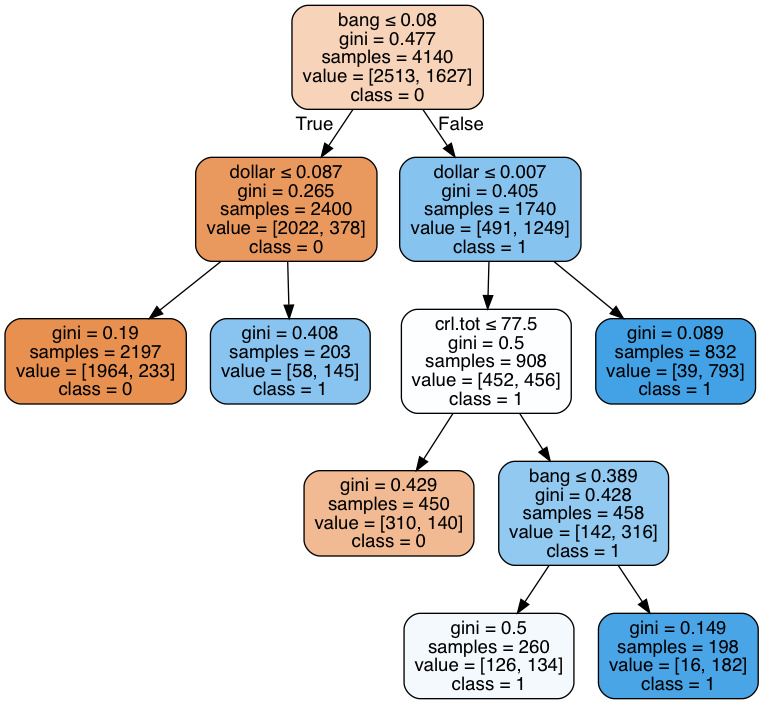
\includegraphics[width = 0.8\linewidth]{data/spam7_opt.png}
            \caption{Измененное дерево решений для примера <<spam7>>}
        \end{figure}

    \section{Набор данных <<nsw74psid1>>}

        Для приведенного набора было построено регрессионное дерево решений (рис. 6)

        \begin{figure}[H]
            \centering
            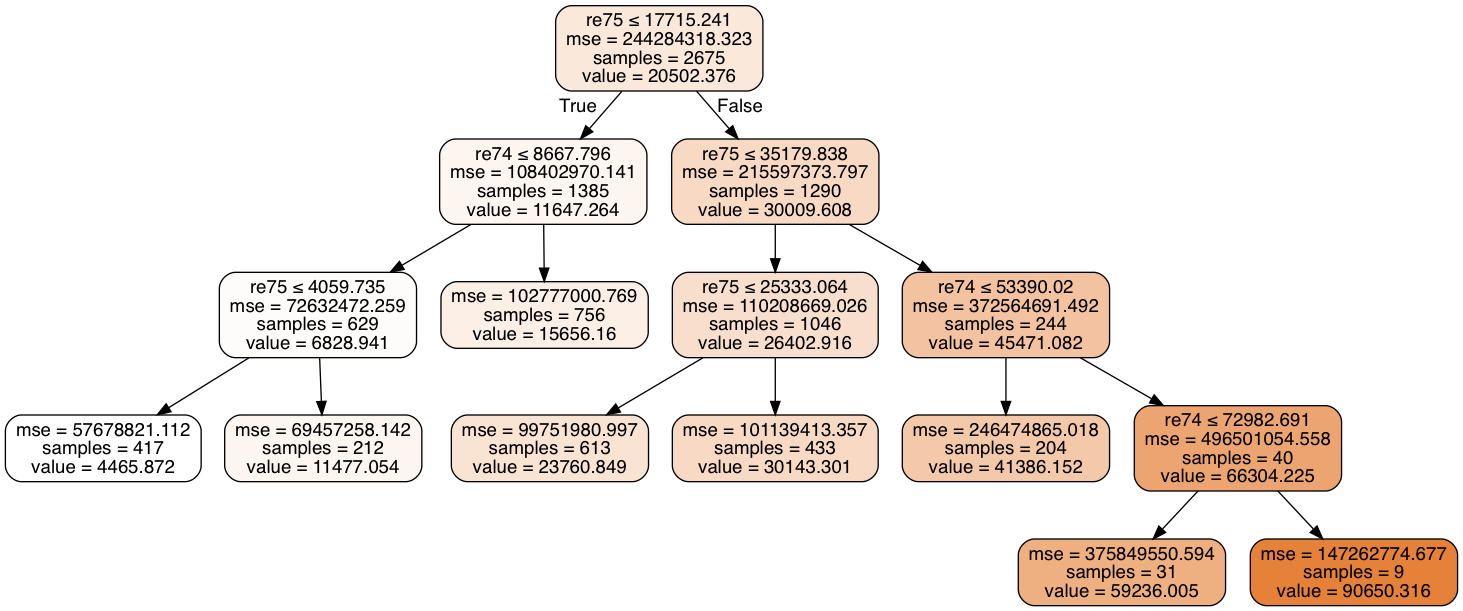
\includegraphics[width = 1.0\linewidth]{data/nsw74psid1.png}
            \caption{Дерево решений для примера <<nsw74psid1>>}
        \end{figure}

    \section{Набор данных <<lenses>>}

        Для набора данных было построено дерево решений (рис. 7).

        \begin{figure}[H]
            \centering
            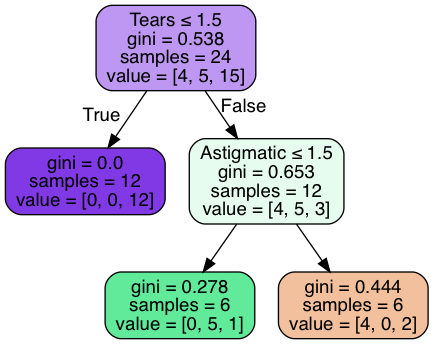
\includegraphics[width = 0.7\linewidth]{data/lenses.png}
            \caption{Дерево решений для примера <<lenses>>}
        \end{figure}

        Также было установлено что при предстарческой дальнозоркости (2), близорукости (1), при наличии астигматизма (2) и сокращенной слезы (1) не следует носить контактные линзы с вероятностью 1.0.

    \section{Набор данных <<svmdata4>>}

        Для набора данных было построено дерево решений (рис. 8).

        \begin{figure}[H]
            \centering
            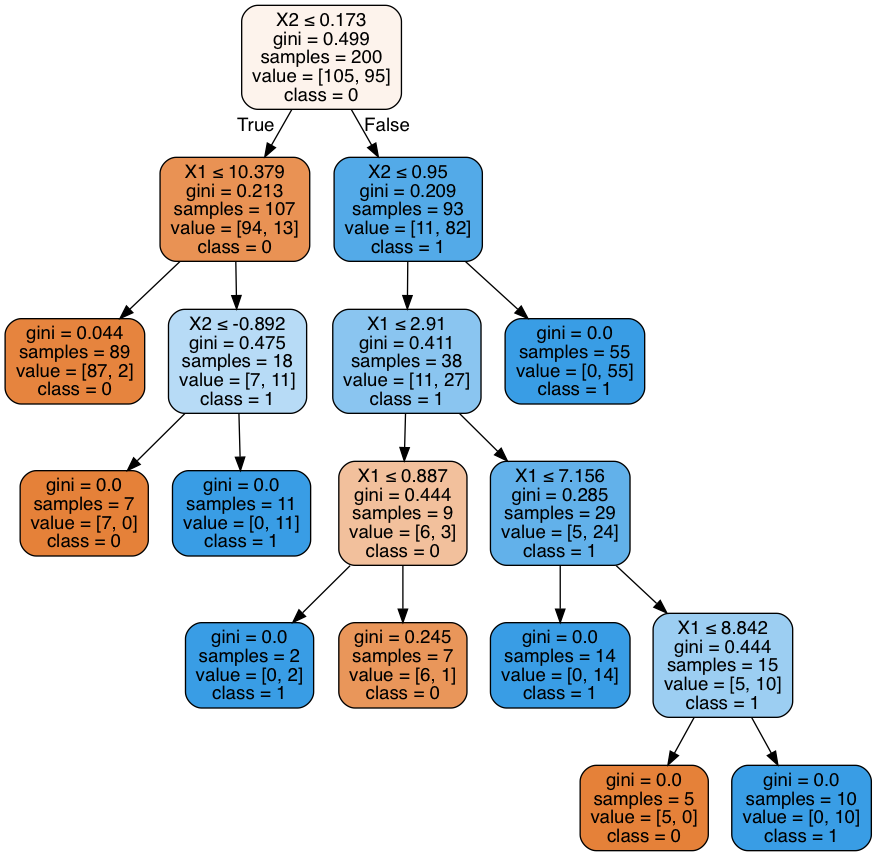
\includegraphics[width = 0.7\linewidth]{data/svmdata.png}
            \caption{Дерево решений для примера <<svmdata4>>}
        \end{figure}

        Вероятность ошибки составила 0.1. Ниже представлена таблица отображающая результаты сравнения полученных данных с исходными.

        \begin{table}[H]
            \centering
            \begin{tabular}{|c|c|c|}
              \hline
                & \textbf{0} & \textbf{1} \\
              \hline
              \textbf{0} & 98 & 3\\
              \hline
              \textbf{1} & 17 & 82 \\
              \hline
            \end{tabular}
            \caption{Сравнение результатов с исходными данными (svmdata4))}
        \end{table}

    \section{Набор данных Titanic}

    В данном примере обучение производилось по всем возможным колонкам, за исключением колонки <<Ticket>>, а также колонки <<SibSp>> и <<Parch>> были заменены на их сумму + 1 (колонка <<FamilySize>>), колонка <<Cabin>> была заменена на колонку с бинарными значениями <<HasCabin>>.

    Полученное дерево изображено ниже (рис. 9)

    \begin{figure}[H]
        \centering
        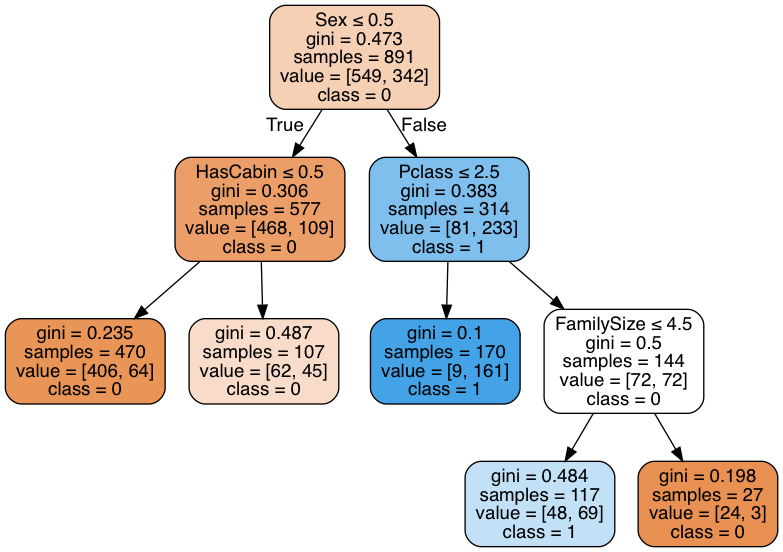
\includegraphics[width = 0.7\linewidth]{data/titanic_tree.png}
        \caption{Дерево решений для примера <<Titanic>>}
    \end{figure}

    Был произведен подсчет величины ошибочной классификации (таблица 9).

    \begin{table}[H]
        \centering
        \begin{tabular}{|c|c|c|}
          \hline
            & \textbf{0} & \textbf{1} \\
          \hline
          \textbf{0} & 266 & 0\\
          \hline
          \textbf{1} & 5 & 147 \\
          \hline
        \end{tabular}
        \caption{Сравнение результатов с исходными данными (Titanic dataset))}
    \end{table}

    Таким образом величина ошибочной классификации в примере составила $\approx0.01$.

\end{document}
